\documentclass[9pt,twoside,lineno]{pnas-new}
% Use the lineno option to display guide line numbers if required.
\usepackage{lipsum} % Required to insert dummy text
\usepackage[version=4]{mhchem}
\usepackage{siunitx}
\usepackage{mathtools}
\templatetype{pnassupportinginfo}

\title{Contiguously-hydrophobic sequences are functionally significant throughout the human exome}
%\corr{* grace.b
\author{Ruchi Lohia, Matthew E.B. Hansen, Grace Brannigan}
\correspondingauthor{Grace Brannigan\\E-mail: grace.brannigan@rutgers.edu}

\begin{document}

%% Comment out or remove this line before generating final copy for submission; this will also remove the warning re: "Consecutive odd pages found".
%\instructionspage  

\maketitle

%% Adds the main heading for the SI text. Comment out this line if you do not have any supporting information text.
%\SItext


%\subsection*{Subhead}
%Type or paste text here. This should be additional explanatory text such as an extended technical description of results, full details of mathematical models, etc.   

%\section*{Heading}
%\subsection*{Subhead}
%Type or paste text here. You may break this section up into subheads as needed (e.g., one section on ``Materials'' and one on ``Methods'').

%\subsection*{Materials}
%Add a materials subsection if you need to.

%\subsection*{Methods}
%Add a methods subsection if you need to.
%\section*{Supplementary Materials}
%%% Each figure should be on its own page
%\clearpage

\begin{figure}[!ht]
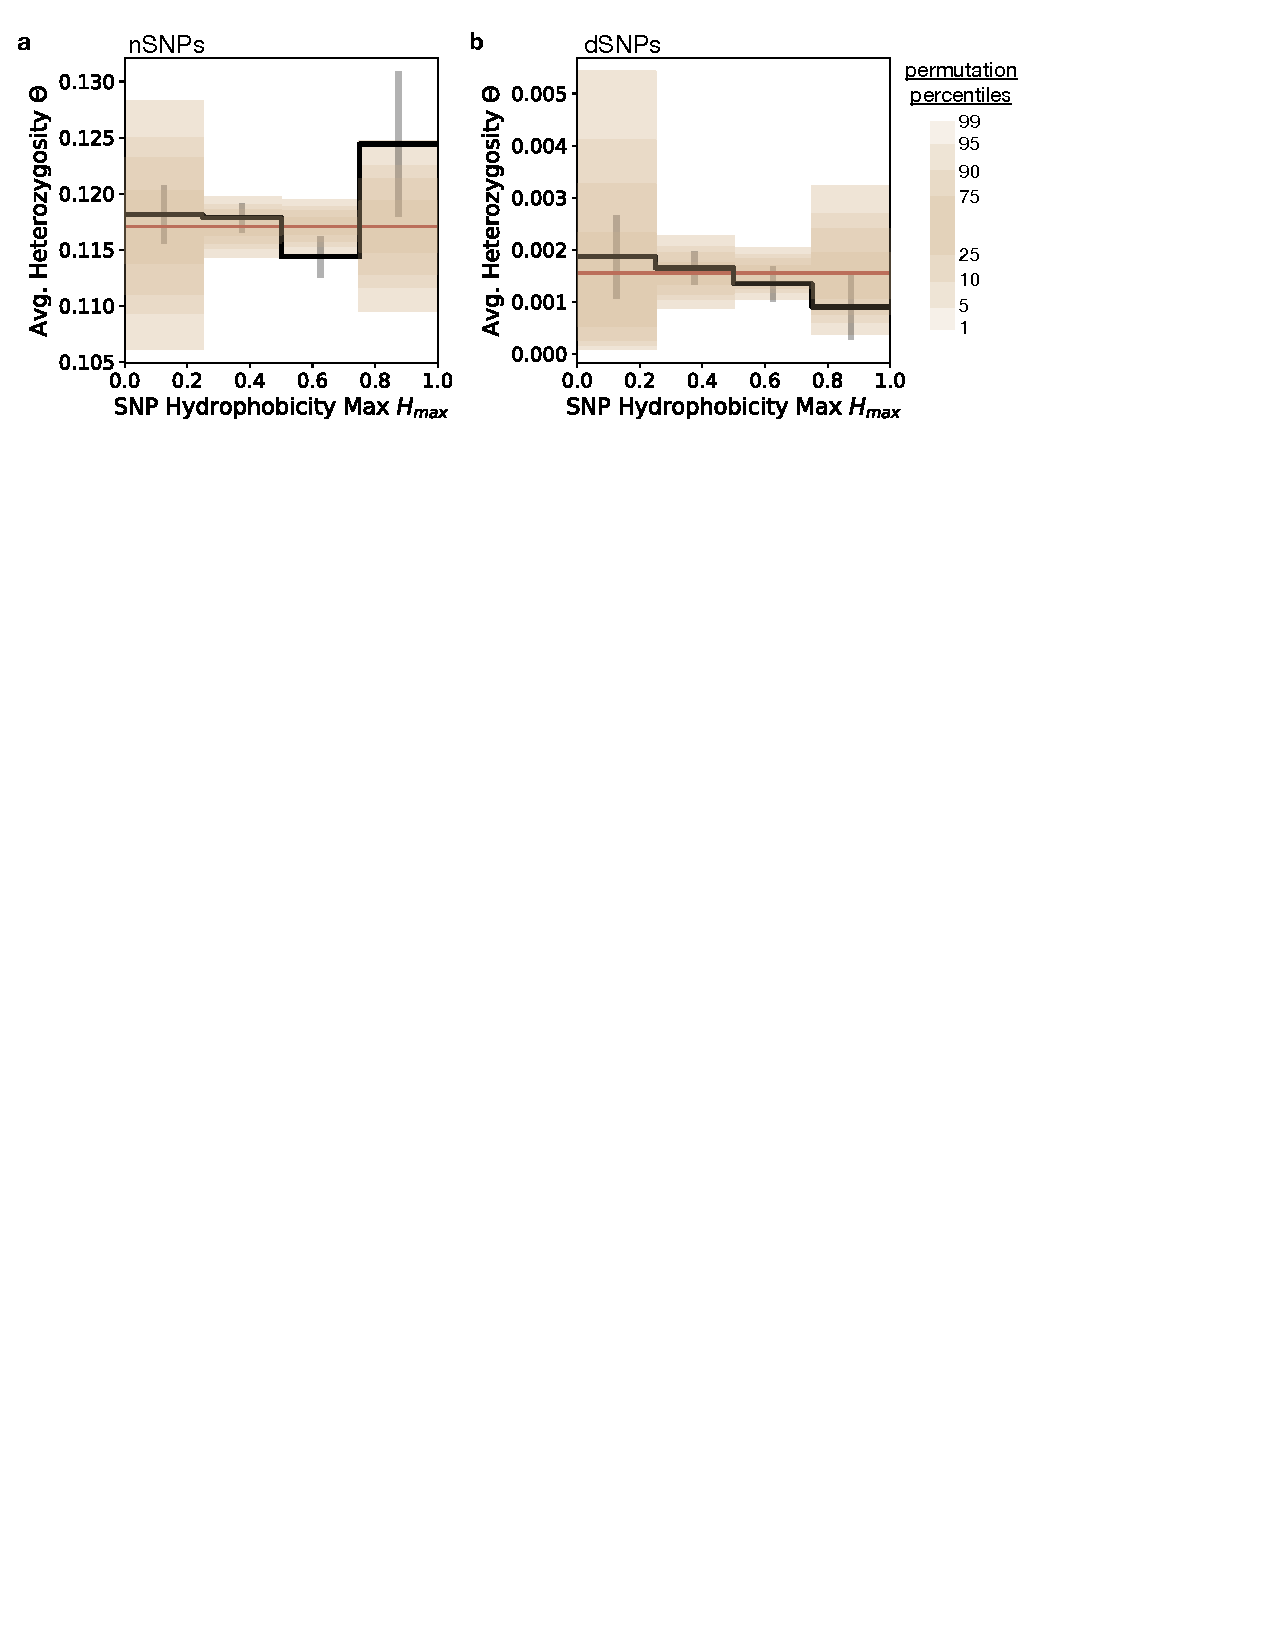
\includegraphics[scale=0.5,width=\textwidth,trim={0 0cm 0 0cm},clip]{Figure_S1.pdf}
\caption{{\bf Heterozygosity of SNPs in East Asians as a function of blob hydrophobicity}. Similar to Fig. 3, but for the gnomAD East Asian population cohort.}
\label{S1} 
\end{figure}

\clearpage

%%% Add this line AFTER all your figures and tables
\FloatBarrier
\dataset{Dataset_S1.txt}{Relative SASA and ``whole-sequence'' blobulation for $L_{\rm min}=4$ and $H^*=0.4$. This is the data used for Fig. 1D, and covers all proteins with a PDB entry, and all residues with a SASA call from DSSP, except transmembrane residues. It is a tab-delimited text file. Each row is the data corresponding to a residue. The columns are: 
\begin{enumerate}
    \item Uniprot\_ID: the UniProt ID for the protein sequence
    \item PDB\_ID: the PDB ID of the structure for that protein
    \item PDB\_chain: the chain identifier for the structure
    \item Res\_ID: the residue number
    \item Res\_name: the one letter amino acid code in the reference sequence
    \item Blob\_class: the hydrophobicity class of the blob this residue resides in, with values ``h'' (h-blob), ``p'' (p-blob), and ``s''(s-blob)
    \item SASA\_relative: the relative SASA value for this residue, based on raw SASA values called by DSSP\citep{Kabsch1983, Touw2015} (see text for normalization)
\end{enumerate}
}

\dataset{Dataset_S2.txt}{Secondary structure and ``whole-sequence'' blobulation for $L_{\rm min}=4$ and $H^*=0.4$. This is the data used for Fig. 1E, and covers all proteins with a PDB entry, and all residues with a secondary structure call from DSSP. This dataset does include transmembrane residues. It is a tab-delimited text file. Each row is the data corresponding to a residue. The columns are: 
\begin{enumerate}
    \item Uniprot\_ID: the UniProt ID for the protein sequence
    \item PDB\_ID: the PDB ID of the structure for that protein
    \item PDB\_chain: the chain identifier for the structure
    \item Res\_ID: the residue number
    \item Res\_name: the one letter amino acid code in the reference sequence
    \item Blob\_class: the hydrophobicity class of the blob this residue resides in, with values ``h'' (h-blob), ``p'' (p-blob), and ``s''(s-blob)
    \item Secondary\_struct\_type: the secondary structure type assigned to this residue, called by DSSP~\citep{Kabsch1983, Touw2015}. The potential values are ``B'' ($\beta$-bridge), ``E'' (extended $\beta$-strand),``G''(3-10 helix), ``H''($\alpha$-helix), ``I''($\pi$-helix), ``S'' (highly curved region),``T'' (turn), and ``-'' (loop or no other assignment). Within Figure 1e of the main text, these subtypes are grouped into three larger classes: helix (G,H,I); strand (B,E); coil (S,T,-)
\end{enumerate}
}

\dataset{Dataset_S3.txt}{This is the unconstrained-length blobulation data per SNP, for all nSNPs and dSNPs, for 21 different hydrophobicity thresholds $H^*=0,0.05,0.1,\dots,1$. This is a tab-delimited text file. Rows correspond to each unique pairing of SNP and hydrophobicity threshold $H^*$. The columns are: 
\begin{enumerate}
    \item ID: a unique peptide variant ID in the format <UniProt\_protein\_ID>:<reference amino acid><residue number><alternative amino acid>
    \item Assoc: the disease-association label, with ``N'' for nSNP and ``D'' for dSNP
    \item Hydrophobicity\_Min: the hydrophobicity threshold $H^*$ used
    \item Blob\_Type\_REF: the blob type for the sequence with the reference amino acid, with values ``h'', ``p'', and ``s''
    \item Blob\_Type\_ALT: the blob type for the sequence with the alternative amino acid, with values ``h'', ``p'', and ``s''
    \item L\_REF: the length of the blob surrounding the variant for the sequence with the reference amino acid
    \item L\_ALT: the length of the blob surrounding the variant for the sequence with the alternative amino acid
\end{enumerate}
} 

\dataset{Dataset_S4.xslx}{Enrichment of dSNPs relative to nSNPs in h blobs for 2D binned hydrophobicity cutoffs and blob lengths. This contains the blobulation count and enrichment data used for Fig. 2. Contains three sheets. Each sheet has the same format. Rows correspond to SNP counts in each 2D bin of blob parameters $\{H^*,L\}$. The columns are: 
\begin{enumerate}
    \item Blob length: the blob length $L$
    \item Hydrophobicity threshold $H^*$: the blob hydrophobicity threshold $H^*$
    \item Number of dSNPs: the number of dSNPs in h-blobs of length $L$ with minimum hydrophobicity $H^*$
    \item Number of nSNPs: the number of nSNPs in h-blobs of length $L$ with minimum hydrophobicity $H^*$
    \item Total number of SNPs: the total number of SNPs in h-blobs of length $L$ with minimum hydrophobicity $H^*$
    \item Enrichment of dSNPs: the enrichment of dSNPs in h-blobs of length $L$ with minimum hydrophobicity $H^*$
    \item p value: the Binomial test two-tailed p-value for the enrichment
\end{enumerate}
Sheet1: all regions, corresponding to Fig. 2D,H. Sheet2: solvated regions, corresponding to Fig. 2E,I. Sheet3: transmembrane regions, corresponding to Fig. 2F,J. }

\dataset{Dataset_S5.txt}{Population frequency data per SNP. This is the data used for Fig. 3 and Fig. S1, and is the subset of variants with a listed rsid in both the UniProt dataset and the gnomAD dataset. It is a tab-delimited text file. Each row is the data corresponding to a UniProt variant with gnomAD frequency data blobulated by the listed hydrophobicity threshold. The columns are: 
\begin{enumerate}
    \item ID: a unique peptide variant ID in the format <UniProt\_protein\_ID>:<reference amino acid><residue number><alternative amino acid>
    \item dbSNP: the variant rsid
    \item Chrom: the chromosome the variant is on
    \item Pos: the base pair position of the variant on the chromosome, in GRCh37 coordinates
    \item Ref: the reference allele nucleotide
    \item Alt: the alternative allele nucleotide
    \item Freq\_Alt\_gnomad:nfe: the frequency of the alternative allele in the gnomAD non-Finnish European frequency data
    \item Freq\_Alt\_gnomad:eas: the frequency of the alternative allele in the gnomAD East Asian frequency data
    \item Het:nfe: the expected population heterozygosity in the non-Finnish European cohort
    \item Het:eas: the expected population heterozygosity in the East Asian cohort
\end{enumerate}
}

\dataset{Dataset_S6.xlsx}{GO enrichment for nSNPs and dSNPs in highly hydrophobic h-blobs, based on the g:Profiler web tool (Raudvere {\it et al}, 2019). Contains two sheets. Each sheet has the same format. Rows correspond to significantly enriched GO terms, where significance is based on the g:SCSS multiple-testing corrected p-value $\leq 0.05$. The columns are: 
\begin{enumerate}
    \item source: the gene ontology database source
    \item term\_name: the GO term
    \item term\_id: GO term ID
    \item adjusted\_p\_value: the g:SCS multiple-testing corrected p-value
    \item negative\_log10\_of\_adjusted\_p\_value: the negative log10 of the adjusted p-value
    \item term\_size: the number of proteins labeled with the GO term
    \item query\_size: the number of proteins in the query set
    \item intersection\_size: the number of query proteins labeled with the GO term
    \item fquery: the fraction of the query set in the intersection
    \item fterm: the fraction of the proteins labeled with the GO term in the intersection
    \item fgeom: the geometric mean of the two fterm and fquery
    \item effective\_domain\_size: the total number of background variants used
    \item intersections: the UniProt IDs for the proteins in the intersection
\end{enumerate}
 Sheet1: GO results for target proteins containing nSNPs with maximum hydrophobicity $H_{max}\geq 0.75$ ($n=635$), compared to a background of all proteins containing an nSNP ($n=10,406$). Sheet2: GO results for target proteins containing dSNPs with maximum hydrophobicity $H_{max}\geq 0.75$ ($n=179$), compared to a background of all proteins containing an nSNP ($n=1,803$). } 




\bibliography{contig_pnas.bib}

\end{document}
